\subsection{Dynamic Power}

\subsubsection*{Spike Activation Per Layer}

Table \ref{tab:spike_activation} shows the mean activation rates ($\zeta$) of each spiking layer inside the \gls{snn} backbone, aggregated across the 200-sample validation subset. 
These layer-wise activation values quantify the metabolic sparsity of the network and were subsequently used to calculate the dynamic power consumption (\glspl{sop}) for each frame in the dataset.

\begin{table}[htbp]
\centering
\begin{tabular}{|l|c|}
\hline
\textbf{Layer Name} & \textbf{Mean Firing Rate ($\zeta$)} \\
\hline
\texttt{stem\_lif} & 20.19\% \\
\texttt{block1.lif1} & 17.93\% \\
\texttt{block1.lif2} & 19.22\% \\
\texttt{block2.lif1} & 0.19\% \\
\texttt{block2.lif2} & 11.11\% \\
\texttt{block3.lif1} & 0.19\% \\
\texttt{block3.lif2} & 0.47\% \\
\texttt{block4.lif1} & 0.58\% \\
\texttt{block4.lif2} & 1.32\% \\
\hline
\end{tabular}
\caption[Layer-Wise Spike Activation Rates]{Mean spike activation rates ($\zeta$) per layer for the \texttt{ULTRA} backbone over the 200-sample experimental set.}
\label{tab:spike_activation}
\end{table}

\subsubsection*{Mean Energy Savings}
\label{subsubsec:mean_energy_savings}

By substituting the empirical layer-wise firing rates ($\zeta$) recorded in Table \ref{tab:spike_activation} into the dynamic power formulation established in Equation \ref{eq:e_snn} (Section \ref{subsec:dynamic_power}), the network's computational operations can be directly translated into theoretical energy consumption in microjoules ($\mu J$). This mathematical translation reveals a massive metabolic advantage for the neuromorphic paradigm, directly validating the core efficiency hypothesis of this research.

Table \ref{tab:energy_statistics} outlines the energy consumption statistics per frame across the 200-sample validation set.
The continuous \gls{cnn} baseline, processing the input uniformly regardless of scene complexity, consumed a massive, static $42,429.21\ \mu J$ per frame with zero variance. 
In contrast, the \texttt{ULTRA} \gls{snn} architecture consumed a mean of only $2,404.98\ \mu J$ per frame, and dipped as low as $2,287.54\ \mu J$ on highly sparse scenes.

\begin{table}[htbp]
\centering
\begin{tabular}{|l|c|c|}
\hline
\textbf{Metric} & \textbf{SNN (\texttt{ULTRA})} & \textbf{CNN Baseline} \\
\hline
Maximum & 2508.22 & 42429.21 \\
Mean & 2404.98 & 42429.21 \\
Median & 2428.74 & 42429.21 \\
Minimum & 2287.54 & 42429.21 \\
Std Dev & 61.17 & 0.00 \\
\hline
\end{tabular}
\caption[Energy Statistics per Frame]{Dynamic energy statistics ($\mu J$ per frame) comparing the \gls{snn} and \gls{cnn} architectures over the 200-sample validation set.}
\label{tab:energy_statistics}
\end{table}

This represents a \textbf{Mean Theoretical Energy Savings of 94.33\%} (with a maximum observed savings of 94.61\% on highly sparse frames). 
This order-of-magnitude reduction definitively validates the core hypothesis of this project: replacing continuous \gls{mac} operations with discrete, event-driven \gls{ac} operations yields profound energy dividends for high-definition automotive perception.

\subsubsection*{Reactive Scalability: The Line of Best Fit}

To empirically validate the hypothesis from Section \ref{subsec:dynamic_power} that the \gls{snn}'s metabolic cost is a dynamic function of activation sparsity, a linear regression analysis was conducted mapping the raw event count ($x$) of each frame against the theoretical energy consumption ($y$ in $\mu J$).

Figure \ref{fig:dynamic_power} illustrates this relationship: the linear regression model yielded the following equation of best fit:
\begin{equation}
    E_{SNN} = 0.001757 \cdot x + 2294.80
\end{equation}
The model demonstrated a strong positive correlation ($R = 0.8668, R^2 = 0.7514$), confirming the highly reactive nature of the spiking backbone. 

Critically, the parameters of this equation map directly to the biological behaviour of the network:
\begin{itemize}
    \item \textbf{The Metabolic Resting State ($y$-intercept):} The constant $2294.80\ \mu J$ represents the architectural overhead---the baseline energy required to simply maintain the membrane potentials across the 11.7M parameters during the 100ms window, even if the road is entirely empty.
    \item \textbf{The Cost of Information (Slope):} The gradient $0.001757\ \mu J$ represents the exact, marginal energy cost of processing a single new event (e.g., a pixel of a car moving). 
\end{itemize}

This proves the \textit{Reactive Scalability} of the architecture. While the \gls{cnn} possesses a static slope of exactly $0$ (burning $42,429\ \mu J$ regardless of whether the frame contains complex traffic or empty asphalt), the \gls{snn} mimics biological neural efficiency by consuming power only in direct proportion to the incoming visual evidence.

\begin{figure}[htbp]
    \centering
    \begin{subfigure}[b]{0.48\textwidth}
        \centering
        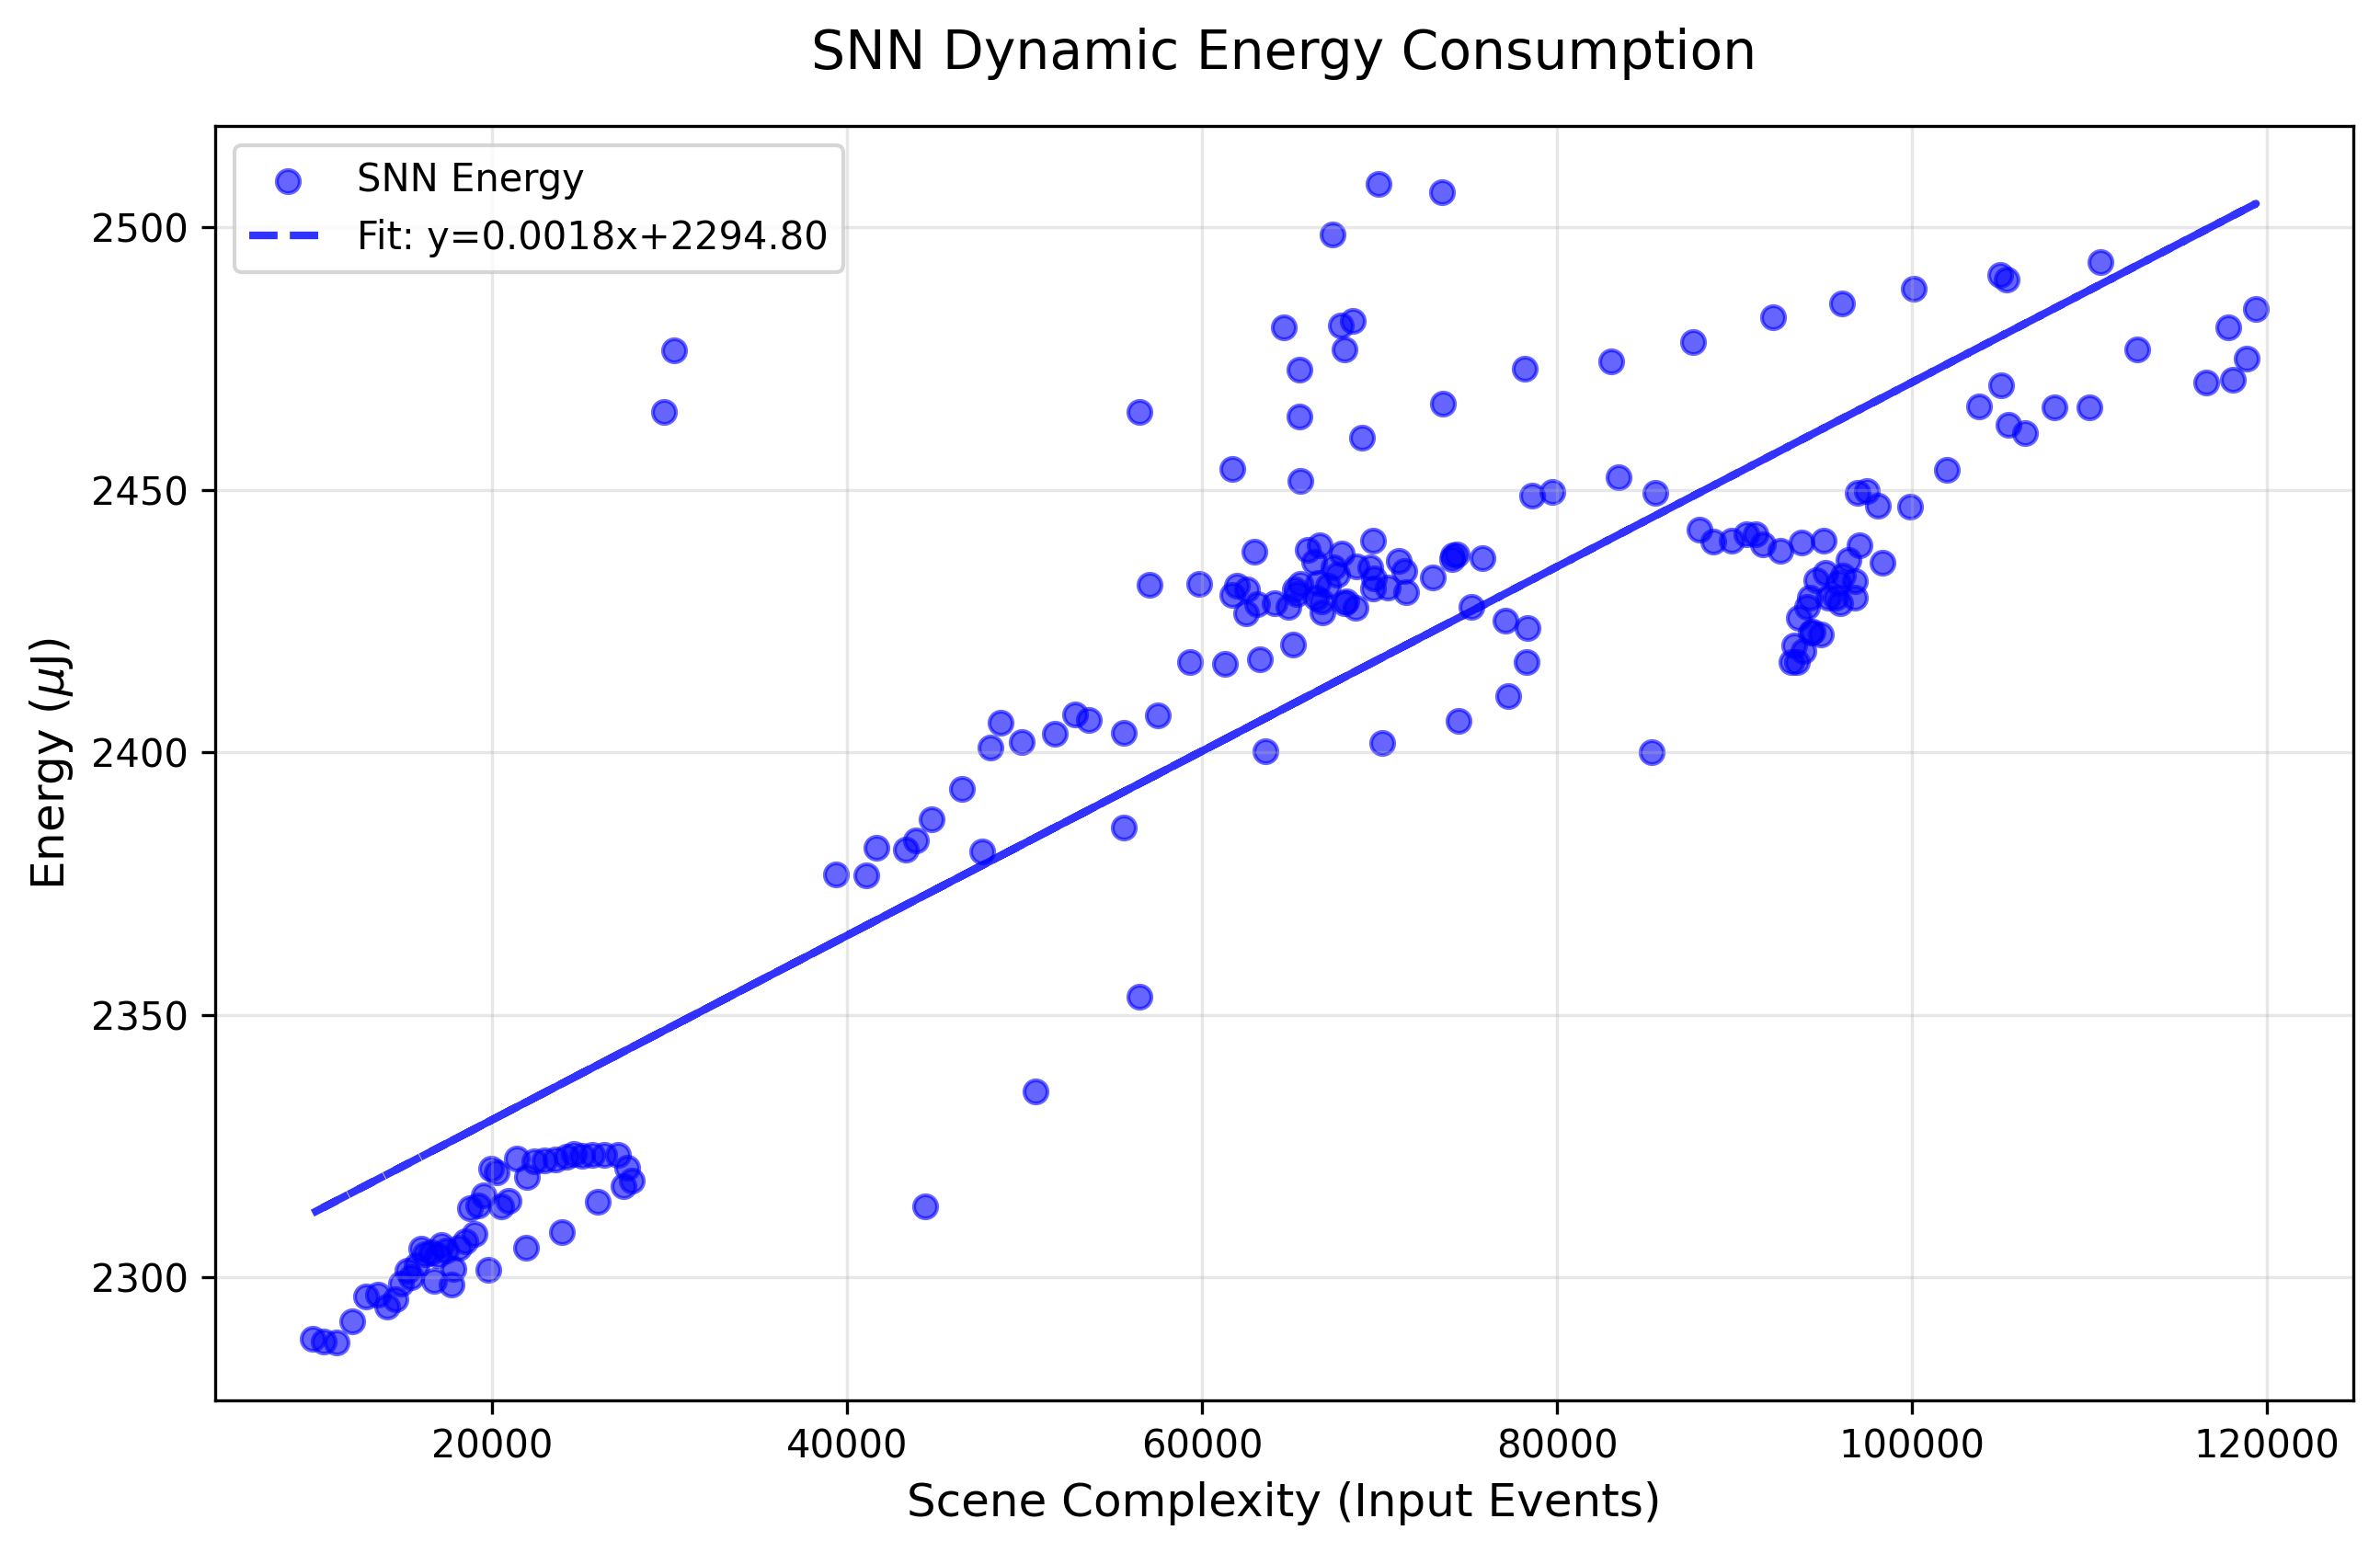
\includegraphics[width=\textwidth]{chapter_3/dnx_results/dynamic_power/exp1_dynamic_power_snn_only.png}
        \caption{SNN Dynamic Power ($\mu J$)}
        \label{fig:dynamic_power_snn}
    \end{subfigure}
    \hfill
    \begin{subfigure}[b]{0.48\textwidth}
        \centering
        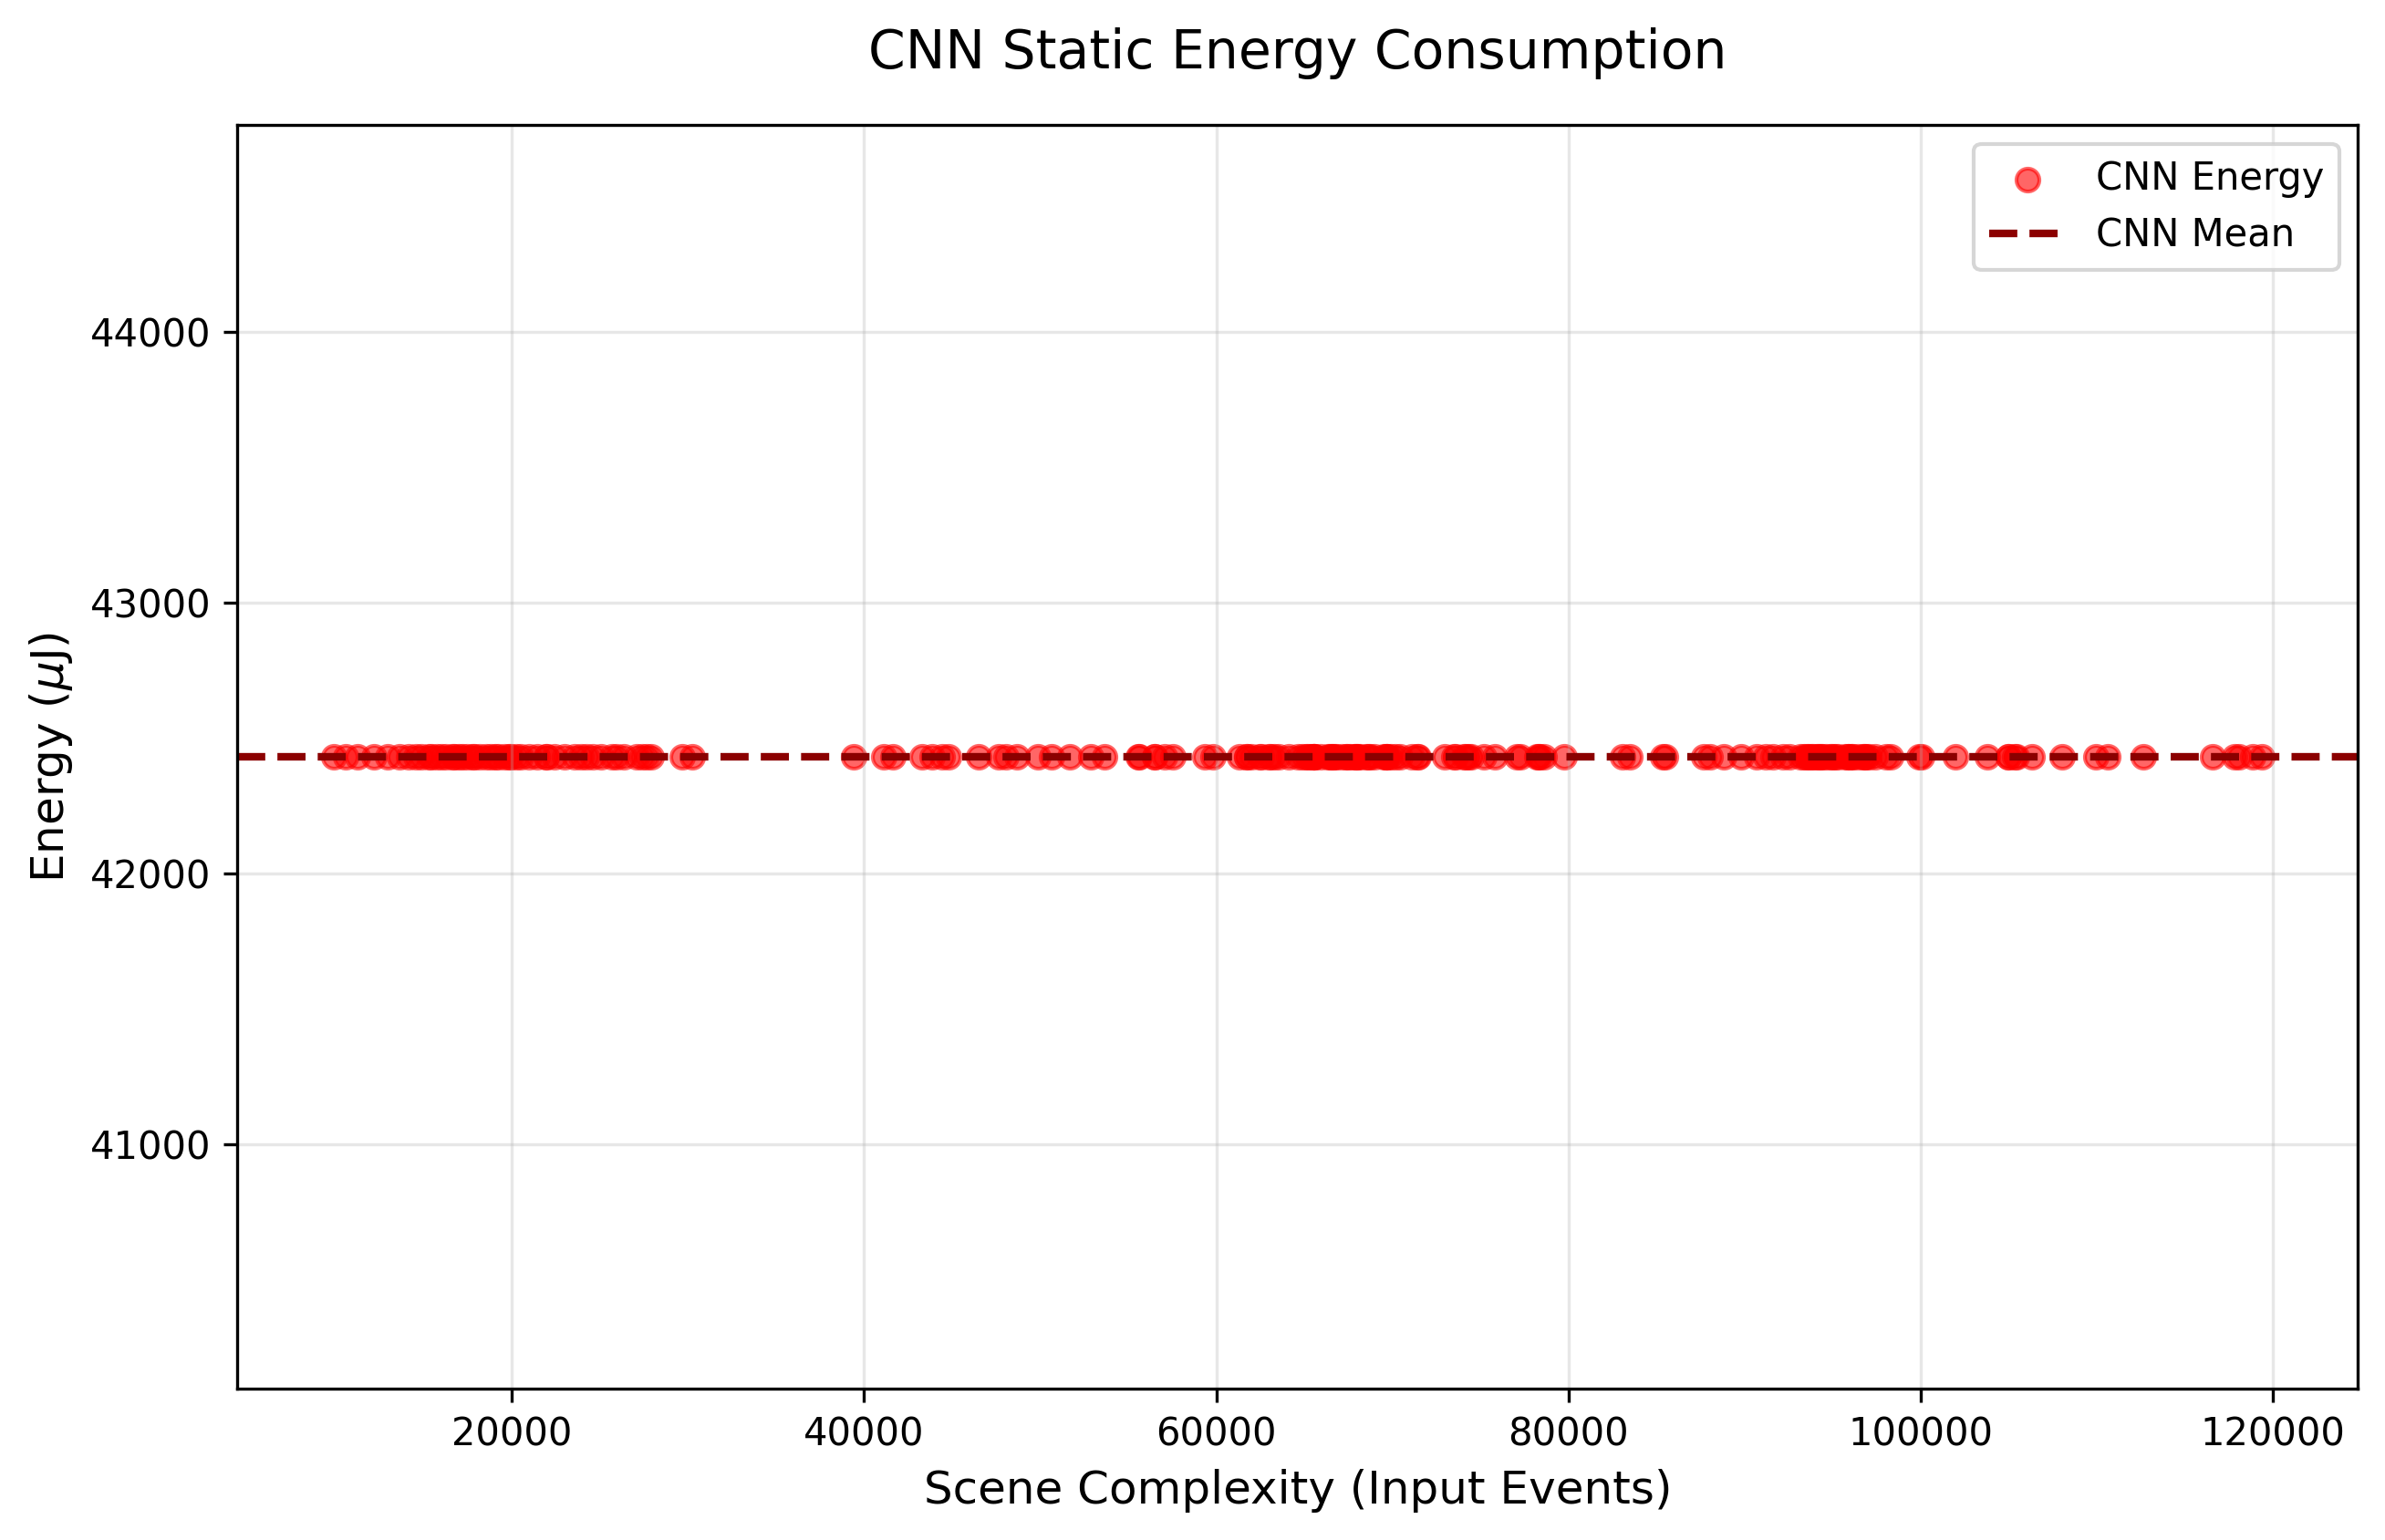
\includegraphics[width=\textwidth]{chapter_3/dnx_results/dynamic_power/exp1_dynamic_power_cnn_only.png}
        \caption{CNN Static Power ($\mu J$)}
        \label{fig:dynamic_power_cnn}
    \end{subfigure}
    
    \vspace{1em}
    
    \begin{subfigure}[b]{0.9\textwidth}
        \centering
        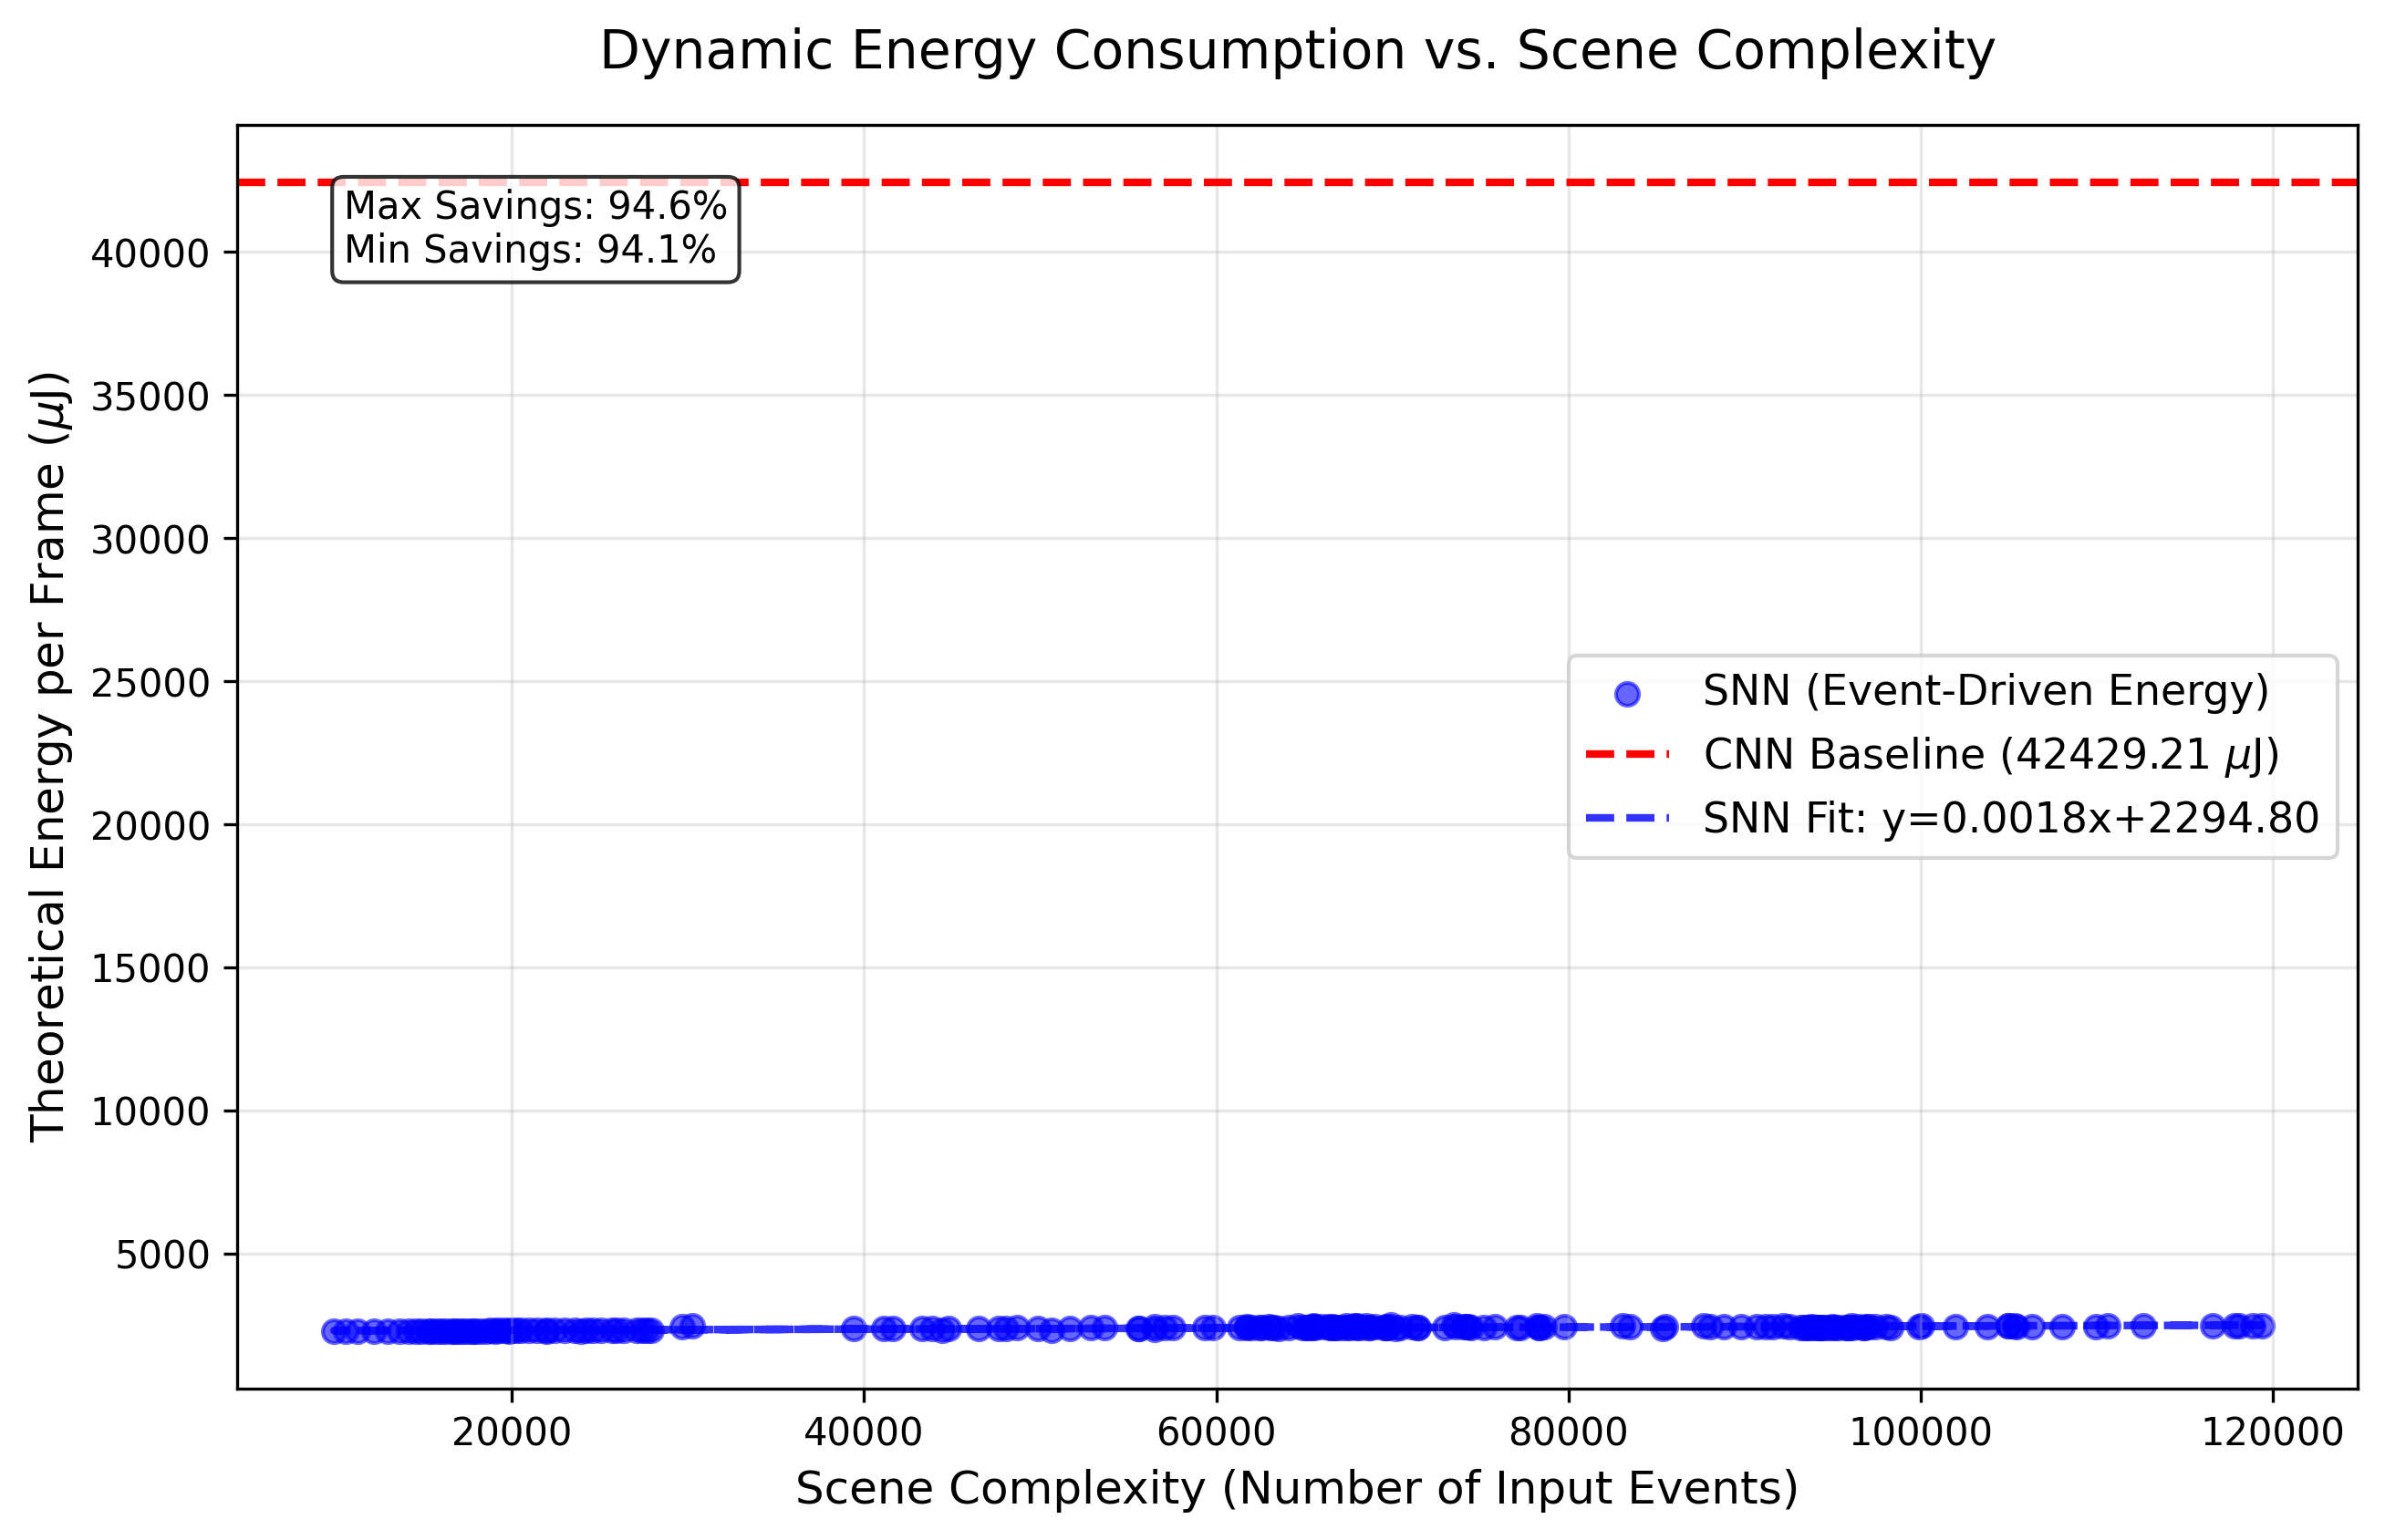
\includegraphics[width=\textwidth]{chapter_3/dnx_results/dynamic_power/exp1_dynamic_power_merged.png}
        \caption{Merged Architecture Comparison}
        \label{fig:dynamic_power_merged}
    \end{subfigure}
    
    \caption[Dynamic Power Consumption vs. Scene Activity]{Comparison of dynamic power consumption ($\mu J$) between the SNN and CNN architectures relative to the raw event count of the input scene. The isolated SNN graph (a) demonstrates strong linear scaling ($R^2 = 0.7514$), validating its event-driven efficiency, whereas the CNN (b) consumes a massive static overhead.}
    \label{fig:dynamic_power}
\end{figure}

\clearpage

\subsubsection*{Mathematical Validation}

To ensure the integrity of the tracking tools and the resulting software-measured data, the theoretical mean power consumption was mathematically verified against the layer-wise operation counts (Table \ref{tab:layer_ops}).

\begin{table}[htbp]
\centering
\begin{tabular}{|l|c|c|c|}
\hline
\textbf{Layer Name} & \textbf{CNN FLOPs ($\times 10^6$)} & \textbf{SNN SOPs ($\times 10^6$)} & \textbf{Sparsity ($\zeta$) (\%)} \\
\hline
\texttt{stem\_lif} & 16.59 & 33.49 & 20.19\% \\
\texttt{block1.lif1} & 265.42 & 476.00 & 17.93\% \\
\texttt{block1.lif2} & 530.84 & 1,020.32 & 19.22\% \\
\texttt{block2.lif1} & 271.32 & 5.02 & 0.19\% \\
\texttt{block2.lif2} & 542.64 & 602.68 & 11.11\% \\
\texttt{block3.lif1} & 1,085.28 & 20.38 & 0.19\% \\
\texttt{block3.lif2} & 2,170.55 & 101.80 & 0.47\% \\
\texttt{block4.lif1} & 2,170.55 & 126.20 & 0.58\% \\
\texttt{block4.lif2} & 2,170.55 & 286.30 & 1.32\% \\
\hline
\textbf{Total Operations} & \textbf{9,223.74} & \textbf{2,672.19} & \textbf{---} \\
\hline
\end{tabular}
\caption[Layer-Wise Operations Comparison]{Comparison of computational operations between the continuous \gls{cnn} and the sparse \gls{snn}. (Values in millions).}
\label{tab:layer_ops}
\end{table}

Substituting these total operations into the methodology formulas (Section \ref{subsec:dynamic_power}) yields:

\begin{itemize}
    \item \textbf{\gls{snn} Power:} $(2672.12\times 10^6) \times 0.9pJ = 2404.97 \mu J$
    \item \textbf{\gls{cnn} Power:} $(9223.74 \times 10^6) \times 4.6pJ = 42429.20 \mu J$
\end{itemize}

These derived values align perfectly with the software-measured empirical means with an error of $\le 0.01\%$,
definitively proving the mathematical integrity of the benchmarking suite.
